\subsection{GCS-Bézier: Hoạch định quỹ đạo với đường cong Bézier}
\label{subsec:GCS-Bézier}

Công thức MICP trong phần trước xây dựng cấu trúc tổng quát cho bài toán đường
đi ngắn nhất trên GCS và kỹ thuật nới lỏng phối cảnh tương ứng. Tuy nhiên, dạng
cụ thể của biến quyết định $x_v$ tại mỗi đỉnh và theo đó, cách biểu diễn đoạn
quỹ đạo trong từng vùng lồi vẫn chưa được đặc tả. Phần này hoàn thiện cầu nối
đó bằng cách tham số hóa mỗi đoạn bằng một đường cong Bézier đa thức, từ đó
định nghĩa khung \emph{GCS-Bézier} cho bài toán hoạch định chuyển động liên tục.

Lựa chọn đường cong Bézier vì tính chất bao lồi (convex hull property) của họ
đường cong này cho phép chuyển ràng buộc an toàn hình học liên tục
$\mathbf{x}(t) \in \mathcal{C}_{\mathrm{free}}$ thành một số hữu hạn ràng buộc
tuyến tính trên các điểm điều khiển nền tảng then chốt để đặt toàn bộ bài
toán về dạng MICP khả giải. Hình~\ref{fig:GCS-Bézier_pipeline} tóm tắt luồng xử
lý tổng thể.

\begin{figure}[H]
    \centering
    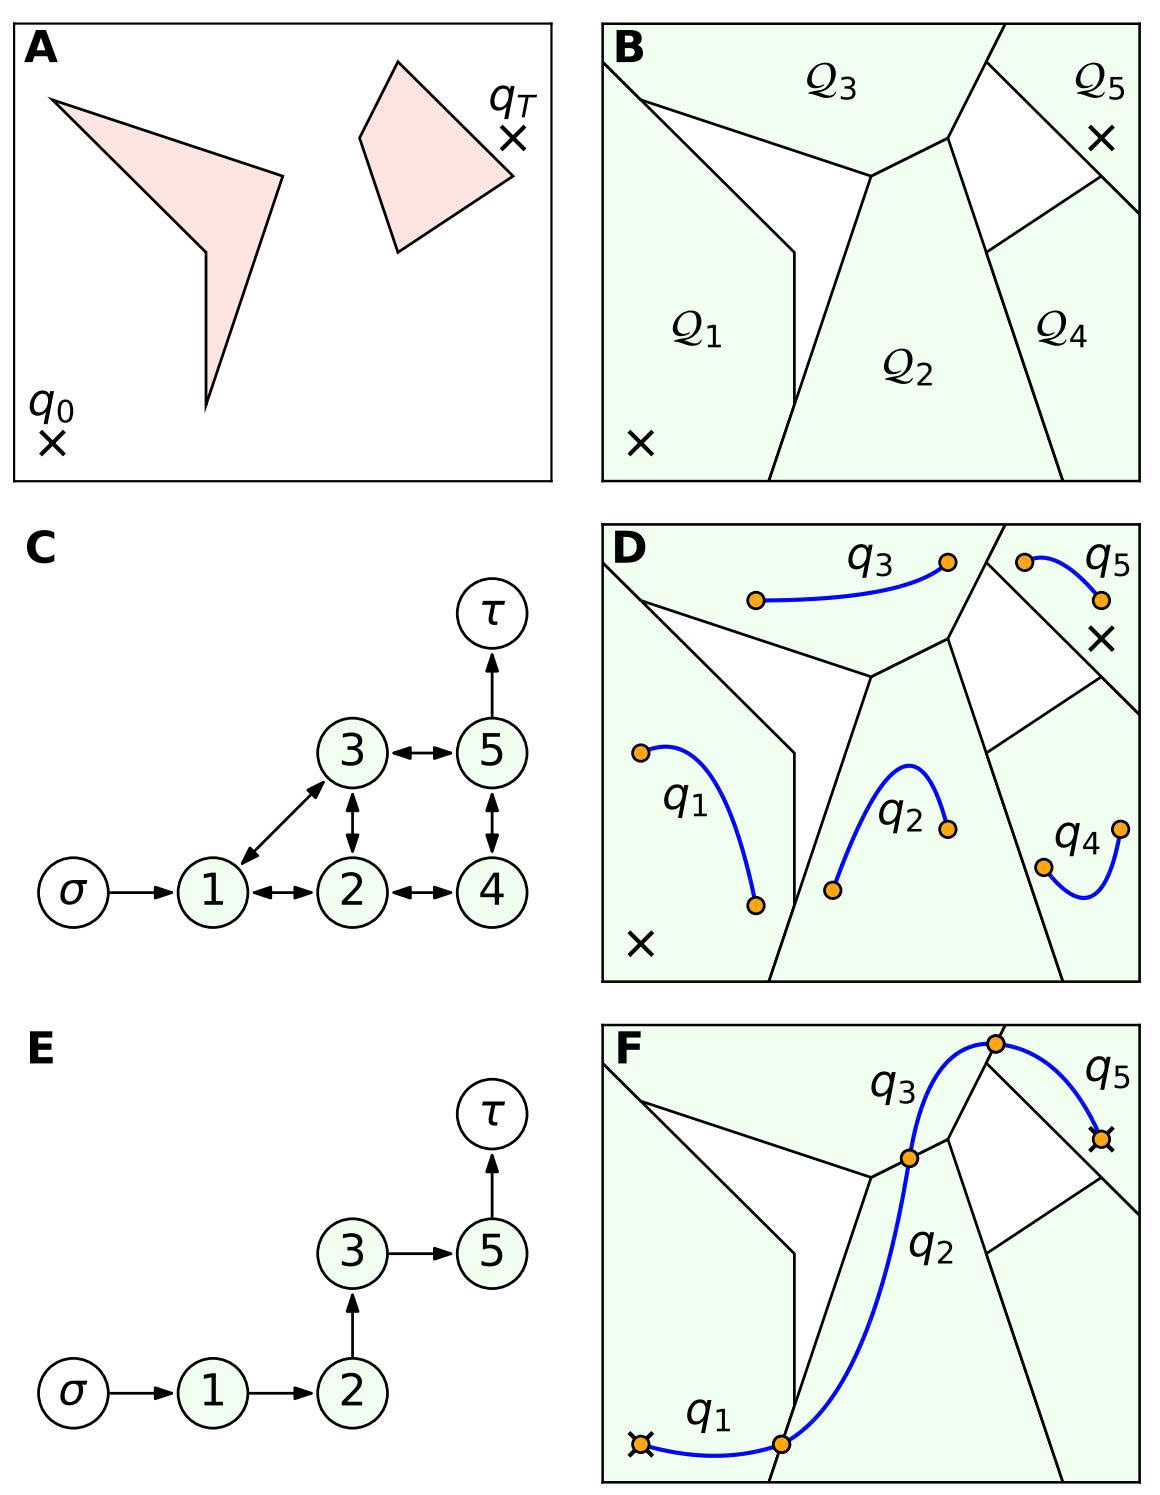
\includegraphics[width=0.8\textwidth]{experiments/image/beziergcs_pipeline.jpg}
    \caption[Motion planning bằng GCS-Bézier trên đồ thị các tập lồi]{%
    \footnotesize
    Bài toán lập kế hoạch chuyển động quanh vật cản được quy về bài toán
    đường đi ngắn nhất trong Graphs of Convex Sets.
    \textbf{(A)} Môi trường gốc gồm các vật cản, cấu hình đầu
    $\mathbf{x}_{\mathrm{start}}$ và cấu hình đích
    $\mathbf{x}_{\mathrm{goal}}$.
    \textbf{(B)} Không gian tự do $\mathcal{C}_{\mathrm{free}}$ được phân hoạch thành các vùng lồi an toàn $\{Q_i\}$.
    \textbf{(C)} Từ quan hệ giao nhau giữa các vùng lồi, xây dựng đồ thị
    $G=(V,E)$, trong đó mỗi đỉnh $i$ tương ứng với một vùng $Q_i$,
    còn hai đỉnh phụ $\sigma$ và $\tau$ biểu diễn cấu hình đầu và cấu hình đích.
    \textbf{(D)} Với mỗi vùng $Q_i$, gán một đoạn quỹ đạo Bézier cục bộ
    $q_i$; các biến quyết định của đoạn này gồm các điểm điều khiển hình học
    và các biến tham số hóa thời gian.
    \textbf{(E)} Việc chọn một đường đi $p$ trên đồ thị sẽ kích hoạt các vùng
    và các cạnh tương ứng, đồng thời kích hoạt các chi phí và ràng buộc ghép nối
    giữa những đoạn Bézier liên tiếp.
    \textbf{(F)} Sau khi giải bài toán MICP hoặc nới lỏng SOCP và làm tròn nghiệm,
    ta thu được quỹ đạo Bézier ghép nối trơn, nằm trong hợp các vùng an toàn lồi
    và nối $\mathbf{x}_{\mathrm{start}}$ tới $\mathbf{x}_{\mathrm{goal}}$.
    }
    \label{fig:GCS-Bézier_pipeline}
\end{figure}

\subsubsection{Lựa chọn đường cong Bézier cho bài toán GCS}
\label{subsubsec:bezier_motivation}

Trong Graphs of Convex Sets, không gian tự do $\mathcal{C}_{\mathrm{free}}$ được biểu
diễn xấp xỉ bằng một họ các vùng lồi $\{Q_v\}_{v \in V}$.
Bài toán motion planning trở thành bài toán chọn một đường đi trên đồ thị $G=(V,E)$
từ $\mathbf{x}_{\mathrm{start}}$ đến $\mathbf{x}_{\mathrm{goal}}$, đồng thời tối ưu
các biến liên tục gắn với các vùng được chọn.
Vì vậy, biểu diễn đường cong trong mỗi vùng $Q_v$ cần thỏa mãn các yêu cầu cấu trúc
xuất phát trực tiếp từ bản chất của bài toán shortest path trên đồ thị vùng lồi.

Thứ nhất, đường cong cần được tham số hóa bởi một số hữu hạn biến quyết định để bài
toán có thể được giải bằng phương pháp số.
Thứ hai, điều kiện để toàn bộ đường cong nằm trong vùng lồi $Q_v$ cần có thể được thay
thế bởi một số hữu hạn ràng buộc lồi trên các biến quyết định đó; nếu không, ràng buộc
an toàn liên tục sẽ không tích hợp được trực tiếp vào bài toán tối ưu.
Thứ ba, điều kiện nối tiếp giữa hai đoạn quỹ đạo trên một cạnh $e=(u,v) \in E$ cần
được biểu diễn bằng các ràng buộc có cấu trúc tuyến tính hoặc song tuyến tính để bảo
toàn tính lồi của bài toán.
Thứ tư, các hàm chi phí như độ dài xấp xỉ, độ mượt, vận tốc hoặc gia tốc cần có thể
được viết dưới dạng lồi hoặc xấp xỉ lồi, để toàn bộ bài toán vẫn nằm trong lớp MICP
giải được.

Đường cong Bézier đáp ứng đồng thời cả bốn yêu cầu trên nhờ tính chất bao lồi.
Trong mỗi vùng $Q_v \subset \mathbb{R}^{n_c}$, một đoạn quỹ đạo được tham số hóa bằng
đường cong Bézier bậc $d$ với $d+1$ điểm điều khiển
$\mathbf{r}_{v,0}, \ldots, \mathbf{r}_{v,d} \in \mathbb{R}^{n_c}$:
\[
    \mathbf{q}_v(s)
    = \sum_{k=0}^{d} B_{k,d}(s)\,\mathbf{r}_{v,k},
    \qquad s \in [0,1].
\]
Vì các hàm cơ sở Bernstein $B_{k,d}(s) = \binom{d}{k}s^k(1-s)^{d-k}$ không âm và
có tổng bằng một trên $[0,1]$, đường cong $\mathbf{q}_v(s)$ là một tổ hợp lồi của
các điểm điều khiển.
Do đó, nếu $\mathbf{r}_{v,k} \in Q_v$ với mọi $k$, thì $\mathbf{q}_v(s) \in Q_v$
với mọi $s \in [0,1]$.

Khi $Q_v$ là đa diện $Q_v = \{x \mid A_v x \le b_v\}$, ràng buộc an toàn liên tục
$\mathbf{q}_v(s) \in Q_v$ được thay thế bởi $d+1$ ràng buộc tuyến tính trên điểm
điều khiển:
\[
    A_v \mathbf{r}_{v,k} \le b_v, \qquad k = 0, \ldots, d.
\]
Đây là lý do chính khiến Bézier phù hợp với GCS: một ràng buộc hình học liên tục
trên toàn bộ đường cong được biến thành các ràng buộc tuyến tính trên điểm điều khiển,
tương thích trực tiếp với cấu trúc MICP hoặc relaxation lồi của bài toán shortest path.

Tại mỗi cạnh $e = (u,v)$, điều kiện liên tục vị trí $\mathbf{r}_{u,d} = \mathbf{r}_{v,0}$
là một ràng buộc tuyến tính trực tiếp trên điểm điều khiển.
Các mức liên tục cao hơn về vận tốc và gia tốc có thể được áp đặt thông qua sai phân
của điểm điều khiển, cũng dưới dạng tuyến tính hoặc song tuyến tính sau khi áp dụng
kỹ thuật phối cảnh.
Nhờ đó, Bézier không chỉ bảo đảm an toàn hình học trong từng vùng lồi cục bộ, mà còn
hỗ trợ ghép nối nhiều đoạn thành một quỹ đạo liên tục từ $\mathbf{x}_{\mathrm{start}}$
đến $\mathbf{x}_{\mathrm{goal}}$.
So với polyline, Bézier cho phép biểu diễn quỹ đạo mượt hơn và đưa ràng buộc động học
vào bài toán; so với spline nội suy hoặc các đường cong đặc thù như Dubins và
Reeds--Shepp, Bézier tương thích trực tiếp hơn với ràng buộc bao lồi và cấu trúc tối
ưu lồi của bài toán shortest path trên graph of convex sets.
Phần tiếp theo đặc tả đầy đủ các tham số và ràng buộc của đoạn quỹ đạo Bézier trong
từng vùng $Q_v$.

\subsubsection{Tham số hóa đường cong Bézier trong vùng lồi}
\label{subsubsec:bezier_param}

Trong mỗi vùng lồi $Q_v \subset \mathbb{R}^{n_c}$ (với $n_c$ là số chiều không
gian cấu hình), đoạn quỹ đạo được tham số hóa bằng một đường cong Bézier bậc
$d$ trên tham số đường $s \in [0,1]$:
\begin{equation}
    \mathbf{q}_v(s)
    = \sum_{k=0}^{d} B_{k,d}(s)\, \mathbf{r}_{v,k},
    \qquad s \in [0,1],
    \label{eq:bezier_curve}
\end{equation}

trong đó $\mathbf{r}_{v,k} \in \mathbb{R}^{n_c}$ là các \emph{điểm điều khiển không gian} và $B_{k,d}(s) = \binom{d}{k} s^k (1-s)^{d-k}$ là đa thức Bernstein
bậc $d$. Hai tính chất cơ bản của cơ sở Bernstein phục vụ trực tiếp bài toán này:
(i)~\textbf{phân hoạch đơn vị}: $\sum_{k=0}^{d} B_{k,d}(s) = 1$, và
(ii)~\textbf{không âm}: $B_{k,d}(s) \ge 0$, với mọi $s \in [0,1]$.
Hai tính chất này khẳng định $\mathbf{q}_v(s)$ là một tổ hợp lồi của các điểm
điều khiển, do đó $\mathbf{q}_v(s) \in \operatorname{conv}\{\mathbf{r}_{v,0},
    \ldots, \mathbf{r}_{v,d}\}$ với mọi $s$.

\begin{proposition}[Bảo đảm an toàn hình học liên tục]
    \label{prop:bezier_safety}
    Nếu tất cả các điểm điều khiển không gian $\mathbf{r}_{v,k} \in Q_v$ với mọi
    $k = 0, \ldots, d$, thì đường cong Bézier $\mathbf{q}_v(s) \in Q_v$ với mọi
    $s \in [0,1]$.
\end{proposition}
\begin{proof}
    Vì $Q_v$ lồi và $\mathbf{q}_v(s)$ là tổ hợp lồi của $\{\mathbf{r}_{v,k}\}_{k=0}^d
        \subset Q_v$, kết quả theo trực tiếp từ định nghĩa tập lồi.
\end{proof}

Mệnh đề~\ref{prop:bezier_safety} có ý nghĩa thực tiễn then chốt: ràng buộc an
toàn liên tục $\mathbf{x}(t) \in Q_v$ được thay thế bởi $d+1$ ràng buộc tuyến
tính $A_v \mathbf{r}_{v,k} \le b_v$ (khi $Q_v = \{x \mid A_v x \le b_v\}$ là đa
diện), cho phép đặt toàn bộ bài toán vào khuôn khổ MICP.

\begin{figure}[htbp]
    \centering
    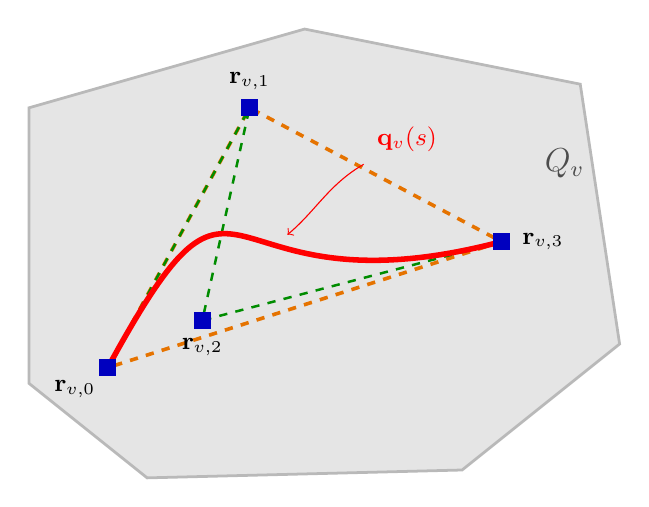
\begin{tikzpicture}[scale=1.0]

        %-- Vùng lồi Q_v (đa giác xám) --
        \fill[gray!20]
        (0,1.0) -- (1.5,-0.2) -- (5.5,-0.1) -- (7.5,1.5) --
        (7.0,4.8) -- (3.5,5.5) -- (0,4.5) -- cycle;
        \draw[gray!55, line width=1pt]
        (0,1.0) -- (1.5,-0.2) -- (5.5,-0.1) -- (7.5,1.5) --
        (7.0,4.8) -- (3.5,5.5) -- (0,4.5) -- cycle;

        %-- Bốn điểm điều khiển: P2 nằm trong conv{P0,P1,P3} --
        %   => đa giác điều khiển P0-P1-P2-P3 không lồi (zigzag)
        %   => bao lồi là tam giác P0-P1-P3
        \coordinate (P0) at (1.0, 1.2);
        \coordinate (P1) at (2.8, 4.5);
        \coordinate (P2) at (2.2, 1.8);   % bên trong conv{P0,P1,P3}
        \coordinate (P3) at (6.0, 2.8);

        %-- Bao lồi conv{r_{v,k}} = tam giác P0-P1-P3 (đường đứt cam) --
        \draw[orange!90!black, dashed, line width=1.3pt]
        (P0) -- (P1) -- (P3) -- cycle;

        %-- Đa giác điều khiển P0→P1→P2→P3 (đường đứt xanh lá) --
        \draw[green!55!black, dashed, line width=0.9pt]
        (P0) -- (P1) -- (P2) -- (P3);

        %-- Đường cong Bézier bậc 3 (đường liền đỏ) --
        %   Nằm trong conv{P0,P1,P2,P3} = tam giác cam
        \draw[red, line width=2pt]
        (P0) .. controls (P1) and (P2) .. (P3);

        %-- Điểm điều khiển: hình vuông xanh đậm --
        \foreach \p in {P0, P1, P2, P3} {
                \node[rectangle, fill=blue!75!black, minimum size=6pt, inner sep=0pt]
                at (\p) {};
            }

        %-- Nhãn các điểm điều khiển --
        \node[font=\small, below left=1pt] at (P0) {$\mathbf{r}_{v,0}$};
        \node[font=\small, above=3pt]      at (P1) {$\mathbf{r}_{v,1}$};
        \node[font=\small, below=3pt]      at (P2) {$\mathbf{r}_{v,2}$};
        \node[font=\small, right=4pt]      at (P3) {$\mathbf{r}_{v,3}$};

        %-- Nhãn vùng Q_v --
        \node[gray!60!black, font=\large] at (6.8, 3.8) {$Q_v$};

        %-- Nhãn đường cong (mũi tên trỏ vào đường cong tại t≈0.6) --
        %   B(0.6) ≈ (3.12, 2.75)
        \node[red, font=\small] (qv) at (4.8, 4.1) {$\mathbf{q}_v(s)$};
        \draw[->, red, thin, shorten >=3pt, shorten <=2pt]
        (qv) to[out=210, in=40] (3.2, 2.82);

    \end{tikzpicture}
    \caption[Đường cong Bézier nằm trong bao lồi của các điểm điều khiển]{%
        Minh họa đường cong Bézier bậc $d=3$ với bốn điểm điều khiển
        $\mathbf{r}_{v,0},\ldots,\mathbf{r}_{v,3}$ nằm trong vùng lồi $Q_v$
        (đa giác xám). Điểm $\mathbf{r}_{v,2}$ được đặt bên trong tam giác
        tạo bởi $\mathbf{r}_{v,0}$, $\mathbf{r}_{v,1}$ và $\mathbf{r}_{v,3}$,
        nên bao lồi của các điểm điều khiển là tam giác đứt cam. Đa giác điều
        khiển đứt xanh có dạng zigzag không-lồi, nhưng đường cong Bézier
        $\mathbf{q}_v(s)$ (đường đỏ) vẫn nằm trọn trong bao lồi cam, chứ không
        phụ thuộc vào hình dạng không-lồi của đa giác điều khiển.}
    \label{fig:bezier_convex_hull}
\end{figure}

Ngoài tọa độ không gian, mỗi đoạn quỹ đạo cần một \emph{hàm thời gian} để ánh
xạ từ tham số $s$ sang thời gian thực $t$. Hàm này cũng được tham số hóa bằng
đường cong Bézier trên các điểm điều khiển thời gian $h_{v,0} \le h_{v,1} \le
    \cdots \le h_{v,d}$:
\begin{equation}
    t_v(s)
    = \sum_{k=0}^{d} B_{k,d}(s)\, h_{v,k},
    \qquad s \in [0,1].
    \label{eq:time_bezier}
\end{equation}
Điều kiện $h_{v,k+1} \ge h_{v,k}$ (hay $\dot{h}_{v,k} := h_{v,k+1} - h_{v,k}
    \ge 0$) đảm bảo $t_v(s)$ đơn điệu tăng; để tránh suy biến, ta đặt
$\dot{h}_{v,k} \ge \varepsilon > 0$ (thực tiễn $\varepsilon = 10^{-6}$).

Đặt $\dot{\mathbf{r}}_{v,k} := \mathbf{r}_{v,k+1} - \mathbf{r}_{v,k}$ là hiệu
điểm điều khiển không gian. Tốc độ tức thời theo thời gian thực tại tham số $s$
được tính bằng quy tắc dây chuyền, và tại các điểm điều khiển $k$, giới hạn vận
tốc $\dot{\mathbf{x}}_v \in D$ (với $D$ là tập lồi có tâm tại gốc) được áp đặt
dưới dạng phối cảnh:
\begin{equation}
    \dot{\mathbf{r}}_{v,k} \in \dot{h}_{v,k}\, D,
    \qquad k = 0, \ldots, d-1,\quad \forall v \in V.
    \label{eq:vel_perspective}
\end{equation}
Đây là dạng tương đương với $\dot{\mathbf{r}}_{v,k}/\dot{h}_{v,k} \in D$ khi
$\dot{h}_{v,k} > 0$, và lồi đồng thời theo $(\dot{\mathbf{r}}_{v,k},
    \dot{h}_{v,k})$ nhờ tính chất hàm phối cảnh bảo toàn tính lồi.
Các ràng buộc tương tự được đặt lên sai phân bậc hai $\ddot{\mathbf{r}}_{v,k}$
để giới hạn gia tốc, và bậc ba để giới hạn độ giật (jerk).

\subsubsection{Ràng buộc liên tục tại điểm chuyển tiếp}
\label{subsubsec:continuity}

Tại mỗi cạnh $e = (u,v) \in E$, đoạn $u$ kết thúc tại $s=1$ và đoạn $v$ bắt đầu
tại $s=0$. Mức độ trơn tru của quỹ đạo ghép nối được điều chỉnh bằng bậc liên
tục yêu cầu.

\paragraph{Liên tục $C^0$ (liên tục vị trí và thời gian).}
\begin{align}
    \mathbf{r}_{u,d} = \mathbf{r}_{v,0},
    \label{eq:c0_pos} \\
    h_{u,d} = h_{v,0}.
    \label{eq:c0_time}
\end{align}
Cả hai đều là ràng buộc \emph{tuyến tính} trực tiếp trên biến điểm điều khiển,
không gây ra bất kỳ khó khăn về tính lồi.

\paragraph{Liên tục $C^1$ (liên tục vận tốc).}
Vận tốc tức thời tại điểm ghép nối phải bằng nhau từ hai phía. Khai triển quy
tắc dây chuyền cho~\eqref{eq:bezier_curve} và~\eqref{eq:time_bezier} tại $s=1$
(đoạn $u$) và $s=0$ (đoạn $v$), ta thu được điều kiện:
\begin{equation}
    \frac{\dot{\mathbf{r}}_{u,d-1}}{\dot{h}_{u,d-1}}
    =
    \frac{\dot{\mathbf{r}}_{v,0}}{\dot{h}_{v,0}}.
    \label{eq:c1_vel}
\end{equation}
Để tránh phép chia, dạng tương đương không phân thức là:
\begin{equation}
    \dot{\mathbf{r}}_{u,d-1}\, \dot{h}_{v,0}
    =
    \dot{\mathbf{r}}_{v,0}\, \dot{h}_{u,d-1}.
    \label{eq:c1_bilinear}
\end{equation}
Ràng buộc~\eqref{eq:c1_bilinear} song tuyến tính (bilinear) giữa các hiệu điểm
điều khiển không gian và thời gian.
Trong khung MICP với nới lỏng phối cảnh, nó được đặt trong tập cạnh
$\mathcal{X}_e$ và trở thành tuyến tính sau khi các biến được co giãn bởi $y_e$.

\paragraph{Liên tục $C^2$ (liên tục gia tốc).}
Đặt $\ddot{\mathbf{r}}_{v,k} := \dot{\mathbf{r}}_{v,k+1} - \dot{\mathbf{r}}_{v,k}$.
Điều kiện gia tốc liên tục tại điểm ghép nối là:
\begin{equation}
    \frac{\ddot{\mathbf{r}}_{u,d-2}}{\bigl(\dot{h}_{u,d-2}\bigr)^2}
    =
    \frac{\ddot{\mathbf{r}}_{v,0}}{\bigl(\dot{h}_{v,0}\bigr)^2},
    \label{eq:c2_acc}
\end{equation}
cũng song tuyến tính và được xử lý tương tự trong cùng khuôn khổ phối cảnh.
Với đường cong bậc $d \ge 3$, điều kiện này thêm vào $n_c$ ràng buộc tuyến tính
sau co giãn cho mỗi cạnh hoạt động.

\begin{figure}[htbp]
    \centering
    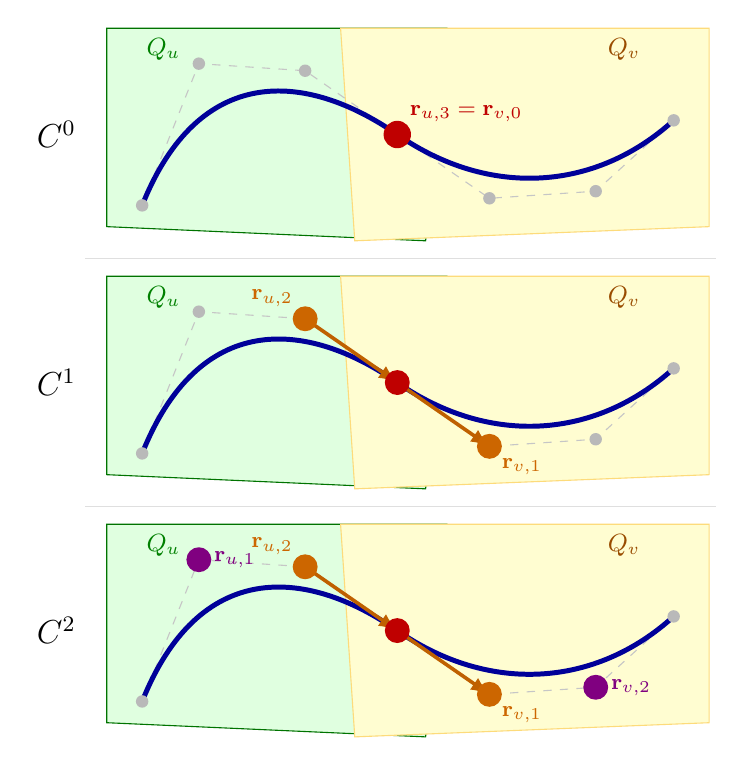
\begin{tikzpicture}[scale=0.9, >=latex]

        % Arrow style for tangent vectors
        \tikzset{tanvec/.style={->, orange!75!black, line width=1.3pt}}

        % Control points (panel-local coords, y in [0,3]):
        %   L0=(1.0,0.5)  L1=(1.8,2.5)  L2=(3.3,2.4)  L3=J=(4.6,1.5)
        %   R0=J=(4.6,1.5) R1=(5.9,0.6) R2=(7.4,0.7)  R3=(8.5,1.7)
        % Tangent at J: L3-L2 = R1-R0 = (1.3,-0.9)  [C1 satisfied by construction]

        %------------------------------------------------------
        % PANEL C^0  (top, shift y=7)
        %------------------------------------------------------
        \begin{scope}[shift={(0,7)}]

            \fill[green!12] (0.5,0.2)--(5.0,0)--(5.3,3)--(0.5,3)--cycle;
            \draw[green!45!black,thin] (0.5,0.2)--(5.0,0)--(5.3,3)--(0.5,3)--cycle;
            \fill[yellow!18] (4.0,0)--(9.0,0.2)--(9.0,3)--(3.8,3)--cycle;
            \draw[yellow!50!orange!50,thin] (4.0,0)--(9.0,0.2)--(9.0,3)--(3.8,3)--cycle;
            \node[green!50!black,font=\small\itshape] at (1.3,2.7) {$Q_u$};
            \node[orange!60!black,font=\small\itshape]  at (7.8,2.7) {$Q_v$};

            \draw[gray!45,dashed,thin]
            (1.0,0.5)--(1.8,2.5)--(3.3,2.4)--(4.6,1.5);
            \draw[gray!45,dashed,thin]
            (4.6,1.5)--(5.9,0.6)--(7.4,0.7)--(8.5,1.7);

            \draw[blue!60!black,line width=1.8pt]
            (1.0,0.5)..controls(1.8,2.5)and(3.3,2.4)..(4.6,1.5);
            \draw[blue!60!black,line width=1.8pt]
            (4.6,1.5)..controls(5.9,0.6)and(7.4,0.7)..(8.5,1.7);

            \foreach \pt in {(1.0,0.5),(1.8,2.5),(3.3,2.4),(5.9,0.6),(7.4,0.7),(8.5,1.7)}
                { \fill[gray!55] \pt circle(2.5pt); }

            % Junction: large red circle
            \fill[red!75!black] (4.6,1.5) circle(5.5pt);
            \node[red!75!black,font=\footnotesize,above right=1pt] at (4.6,1.5)
            {$\mathbf{r}_{u,3} = \mathbf{r}_{v,0}$};

            \node[font=\large\bfseries,anchor=east] at (0.2,1.5) {$C^0$};
        \end{scope}

        %------------------------------------------------------
        % PANEL C^1  (middle, shift y=3.5)
        %------------------------------------------------------
        \begin{scope}[shift={(0,3.5)}]

            \fill[green!12] (0.5,0.2)--(5.0,0)--(5.3,3)--(0.5,3)--cycle;
            \draw[green!45!black,thin] (0.5,0.2)--(5.0,0)--(5.3,3)--(0.5,3)--cycle;
            \fill[yellow!18] (4.0,0)--(9.0,0.2)--(9.0,3)--(3.8,3)--cycle;
            \draw[yellow!50!orange!50,thin] (4.0,0)--(9.0,0.2)--(9.0,3)--(3.8,3)--cycle;
            \node[green!50!black,font=\small\itshape] at (1.3,2.7) {$Q_u$};
            \node[orange!60!black,font=\small\itshape]  at (7.8,2.7) {$Q_v$};

            \draw[gray!45,dashed,thin]
            (1.0,0.5)--(1.8,2.5)--(3.3,2.4)--(4.6,1.5);
            \draw[gray!45,dashed,thin]
            (4.6,1.5)--(5.9,0.6)--(7.4,0.7)--(8.5,1.7);

            \draw[blue!60!black,line width=1.8pt]
            (1.0,0.5)..controls(1.8,2.5)and(3.3,2.4)..(4.6,1.5);
            \draw[blue!60!black,line width=1.8pt]
            (4.6,1.5)..controls(5.9,0.6)and(7.4,0.7)..(8.5,1.7);

            % Non-highlighted: r_{u,0}, r_{u,1}, r_{v,2}, r_{v,3}
            \foreach \pt in {(1.0,0.5),(1.8,2.5),(7.4,0.7),(8.5,1.7)}
                { \fill[gray!55] \pt circle(2.5pt); }

            % Tangent vectors L2->J and J->R1 (collinear, same direction)
            \draw[tanvec] (3.3,2.4) -- (4.6,1.5);
            \draw[tanvec] (4.6,1.5) -- (5.9,0.6);

            % C1 points: r_{u,2} and r_{v,1} (orange)
            \fill[orange!80!black] (3.3,2.4) circle(5pt);
            \fill[orange!80!black] (5.9,0.6) circle(5pt);

            % Junction (red, drawn last so it sits on top)
            \fill[red!75!black] (4.6,1.5) circle(5pt);

            \node[orange!80!black,font=\footnotesize,above left=1pt] at (3.3,2.4)
            {$\mathbf{r}_{u,2}$};
            \node[orange!80!black,font=\footnotesize,below right=1pt] at (5.9,0.6)
            {$\mathbf{r}_{v,1}$};

            \node[font=\large\bfseries,anchor=east] at (0.2,1.5) {$C^1$};
        \end{scope}

        %------------------------------------------------------
        % PANEL C^2  (bottom, shift y=0)
        %------------------------------------------------------
        \begin{scope}[shift={(0,0)}]

            \fill[green!12] (0.5,0.2)--(5.0,0)--(5.3,3)--(0.5,3)--cycle;
            \draw[green!45!black,thin] (0.5,0.2)--(5.0,0)--(5.3,3)--(0.5,3)--cycle;
            \fill[yellow!18] (4.0,0)--(9.0,0.2)--(9.0,3)--(3.8,3)--cycle;
            \draw[yellow!50!orange!50,thin] (4.0,0)--(9.0,0.2)--(9.0,3)--(3.8,3)--cycle;
            \node[green!50!black,font=\small\itshape] at (1.3,2.7) {$Q_u$};
            \node[orange!60!black,font=\small\itshape]  at (7.8,2.7) {$Q_v$};

            \draw[gray!45,dashed,thin]
            (1.0,0.5)--(1.8,2.5)--(3.3,2.4)--(4.6,1.5);
            \draw[gray!45,dashed,thin]
            (4.6,1.5)--(5.9,0.6)--(7.4,0.7)--(8.5,1.7);

            \draw[blue!60!black,line width=1.8pt]
            (1.0,0.5)..controls(1.8,2.5)and(3.3,2.4)..(4.6,1.5);
            \draw[blue!60!black,line width=1.8pt]
            (4.6,1.5)..controls(5.9,0.6)and(7.4,0.7)..(8.5,1.7);

            % Gray: r_{u,0}, r_{v,3}
            \foreach \pt in {(1.0,0.5),(8.5,1.7)}
                { \fill[gray!55] \pt circle(2.5pt); }

            % C2 extra points: r_{u,1} and r_{v,2} (violet)
            \fill[violet] (1.8,2.5) circle(5pt);
            \fill[violet] (7.4,0.7) circle(5pt);

            % Tangent vectors (orange, same as C1)
            \draw[tanvec] (3.3,2.4) -- (4.6,1.5);
            \draw[tanvec] (4.6,1.5) -- (5.9,0.6);

            % C1 points (orange)
            \fill[orange!80!black] (3.3,2.4) circle(5pt);
            \fill[orange!80!black] (5.9,0.6) circle(5pt);

            % Junction (red)
            \fill[red!75!black] (4.6,1.5) circle(5pt);

            \node[violet,font=\footnotesize,right=2pt] at (1.8,2.5)
            {$\mathbf{r}_{u,1}$};
            \node[violet,font=\footnotesize,right=2pt] at (7.4,0.7)
            {$\mathbf{r}_{v,2}$};
            \node[orange!80!black,font=\footnotesize,above left=1pt] at (3.3,2.4)
            {$\mathbf{r}_{u,2}$};
            \node[orange!80!black,font=\footnotesize,below right=1pt] at (5.9,0.6)
            {$\mathbf{r}_{v,1}$};

            \node[font=\large\bfseries,anchor=east] at (0.2,1.5) {$C^2$};
        \end{scope}

        % Thin horizontal rules separating the three panels
        \draw[gray!25,very thin] (0.2,3.25) -- (9.1,3.25);
        \draw[gray!25,very thin] (0.2,6.75) -- (9.1,6.75);

    \end{tikzpicture}
    \caption[Ràng buộc liên tục $C^0$, $C^1$, $C^2$ tại điểm chuyển tiếp]{%
        Minh họa hai đoạn Bézier bậc $d=3$ nối nhau trên hai vùng
        $Q_u$ và $Q_v$. Ở mức $C^0$, hai đoạn chỉ cần gặp nhau tại cùng một
        điểm nối $\mathbf{r}_{u,3}=\mathbf{r}_{v,0}$, được đánh dấu bằng
        chấm đỏ. Ở mức $C^1$, các điểm điều khiển lân cận
        $\mathbf{r}_{u,2}$ và $\mathbf{r}_{v,1}$ được sắp xếp sao cho hai
        tiếp tuyến tại điểm nối cùng hướng, tạo chuyển tiếp trơn hơn. Ở mức
        $C^2$, các điểm xa hơn $\mathbf{r}_{u,1}$ và $\mathbf{r}_{v,2}$
        cũng tham gia ràng buộc, giúp hai đoạn khớp thêm về độ uốn tại điểm nối.}
    \label{fig:continuity_conditions}
\end{figure}

\subsubsection{Bài toán GCS-Bézier hoàn chỉnh}
\label{subsubsec:GCS-Bézier_complete}

Kết hợp cấu trúc luồng mạng từ~\eqref{eq:micp_formulation}, tham số hóa Bézier,
và các ràng buộc liên tục trên đây, bài toán GCS-Bézier đầy đủ được phát biểu
dưới dạng MICP. Tại mỗi đỉnh $v \in V$, biến quyết định là:
\[
    x_v = \bigl(\mathbf{r}_{v,0}, \ldots, \mathbf{r}_{v,d},\;
    h_{v,0}, \ldots, h_{v,d}\bigr)
    \;\in\; \mathbb{R}^{(n_c + 1)(d+1)}.
\]

\begin{subequations}
    \label{eq:GCS-Bézier_full}
    \begin{align}
        \underset{y,\; x}{\mathrm{minimize}} \quad
         & \sum_{e=(u,v) \in E} \tilde{\ell}_e\!\bigl(
        (z_{e,u},\, z_{e,v}),\; y_e
        \bigr)
        \label{eq:bgcs_obj}                                                                  \\
        \mathrm{subject\ to} \quad
         & \sum_{e \in \mathcal{E}^+(u)} y_e - \sum_{e \in \mathcal{E}^-(u)} y_e = \delta_u,
        \quad \forall u \in V,
        \label{eq:bgcs_flow}                                                                 \\
         & \mathbf{r}_{v,k} \in Q_v,
        \quad k = 0, \ldots, d,\quad \forall v \in V,
        \label{eq:bgcs_geo}                                                                  \\
         & \dot{h}_{v,k} \ge \varepsilon,
        \quad k = 0, \ldots, d-1,\quad \forall v \in V,
        \label{eq:bgcs_mono}                                                                 \\
         & \dot{\mathbf{r}}_{v,k} \in \dot{h}_{v,k}\, D,
        \quad k = 0, \ldots, d-1,\quad \forall v \in V,
        \label{eq:bgcs_vel}                                                                  \\
         & h_{v,0} \ge 0,\quad h_{v,d} \le T_{\max},\quad \forall v \in V,
        \label{eq:bgcs_time}                                                                 \\
         & \mathbf{r}_{u,d} = \mathbf{r}_{v,0},\quad
        h_{u,d} = h_{v,0},
        \quad \forall e=(u,v) \in E,
        \label{eq:bgcs_c0}                                                                   \\
         & \dot{\mathbf{r}}_{u,d-1}\, \dot{h}_{v,0}
        = \dot{\mathbf{r}}_{v,0}\, \dot{h}_{u,d-1},
        \quad \forall e=(u,v) \in E,
        \label{eq:bgcs_c1}                                                                   \\
         & \mathbf{r}_{s,0} = \mathbf{x}_{\mathrm{start}},\quad
        h_{s,0} = 0,\quad
        \mathbf{r}_{t,d} = \mathbf{x}_{\mathrm{goal}},
        \label{eq:bgcs_bc}                                                                   \\
         & y_e \in \{0,1\},\quad \forall e \in E.
        \label{eq:bgcs_bin}
    \end{align}
\end{subequations}

Ràng buộc~\eqref{eq:bgcs_geo} là tuyến tính (khi $Q_v$ là đa diện), bảo đảm an
toàn hình học liên tục qua tính chất bao lồi của Bézier. Ràng
buộc~\eqref{eq:bgcs_vel} mã hóa giới hạn vận tốc dưới dạng phối cảnh, lồi đồng
thời theo $(\dot{\mathbf{r}}_{v,k}, \dot{h}_{v,k})$. Ràng buộc liên tục
$C^1$~\eqref{eq:bgcs_c1} là song tuyến tính; sau khi thay các biến bằng dạng co
giãn $z_{e,\cdot} = y_e\, x_\cdot$ theo kỹ thuật phối cảnh, ràng buộc này trở
thành tuyến tính trong biến nâng bậc. Điều kiện biên~\eqref{eq:bgcs_bc} áp đặt
vị trí đầu và cuối tại đỉnh nguồn $s$ và đỉnh đích $t$.

Sau khi áp dụng nới lỏng phối cảnh toàn bộ, bài toán~\eqref{eq:GCS-Bézier_full}
trở thành Quy hoạch Nón Bậc hai Nguyên Hỗn hợp (MI-SOCP), có thể giải bởi các
bộ giải SOCP/MISOCP thương mại (Gurobi, Mosek) hoặc mã nguồn mở với bảo đảm tính tối ưu toàn cục trong giới hạn dung sai nguyên.

\subsubsection{Ví dụ minh họa: GCS-Bézier bậc hai trong không gian 2D}
\label{subsubsec:GCS-Bézier_example2d}

Để minh họa khung GCS-Bézier, xét bài toán tìm đường đi hình học cho robot điểm
trong không gian cấu hình hai chiều $\mathbb{R}^2$. Không gian tự do
$\mathcal{C}_{\mathrm{free}}$ được phân hoạch thành các vùng an toàn lồi
$\{Q_v\}_{v\in V}$, trong đó mỗi vùng $Q_v$ không giao với vật cản. Từ các vùng
này, ta xây dựng đồ thị GCS $G=(V,E)$, với mỗi đỉnh $v$ tương ứng một vùng lồi
$Q_v$, và mỗi cạnh $(u,v)$ biểu diễn khả năng chuyển tiếp giữa hai vùng kề nhau.

Mục tiêu của bài toán là tìm một đường đi rời rạc từ nguồn $\sigma$ đến đích
$\tau$ trên đồ thị $G$, đồng thời tìm một đường cong hình học liên tục nằm hoàn
toàn trong các vùng lồi được chọn. Với mỗi vùng $Q_v$ được kích hoạt, gán một
đoạn Bézier bậc hai
\begin{equation}
    q_v(\theta)
    =
    (1-\theta)^2 q_v^s
    + 2(1-\theta)\theta q_v^m
    + \theta^2 q_v^t,
    \qquad \theta\in[0,1],
\end{equation}
trong đó $q_v^s,q_v^m,q_v^t\in\mathbb{R}^2$ lần lượt là điểm điều khiển đầu,
giữa và cuối của đoạn cong trong vùng $Q_v$.

Do đường Bézier nằm trong bao lồi của các điểm điều khiển, ràng buộc an toàn
hình học có thể được áp đặt bằng điều kiện
\begin{equation}
    q_v^s,\;q_v^m,\;q_v^t \in Q_v.
\end{equation}
Khi đó suy ra
\begin{equation}
    q_v(\theta)\in Q_v,\qquad \forall \theta\in[0,1],
\end{equation}
nên toàn bộ đoạn cong nằm trong vùng an toàn tương ứng.

Với mỗi cạnh được chọn $e=(u,v)$, hai đoạn Bézier kề nhau được ghép bằng ràng
buộc liên tục vị trí
\begin{equation}
    q_u^t = q_v^s.
\end{equation}
Nếu cần đường đi trơn hơn, có thể thêm ràng buộc liên tục tiếp tuyến hình học
\begin{equation}
    q_u^t - q_u^m
    =
    q_v^m - q_v^s.
\end{equation}
Ràng buộc này chỉ bảo đảm độ trơn hình học của đường cong, chưa phải ràng buộc
vận tốc theo thời gian thực.

Một hàm chi phí đơn giản cho đường đi hình học là tổng độ dài xấp xỉ của các đa
giác điều khiển:
\begin{equation}
    J
    =
    \sum_{v\in V_{\mathrm{act}}}
    \left(
    \|q_v^m-q_v^s\|_2
    +
    \|q_v^t-q_v^m\|_2
    \right).
\end{equation}
Khi đó bài toán GCS-Bézier bậc hai có thể viết gọn dưới dạng
\begin{equation}
    \begin{aligned}
        \min_{\{y_e\},\,\{q_v^s,q_v^m,q_v^t\}}
        \quad
         & \sum_{v\in V_{\mathrm{act}}}
        \left(
        \|q_v^m-q_v^s\|_2
        +
        \|q_v^t-q_v^m\|_2
        \right)                                                                   \\[1mm]
        \mathrm{s.t.}\quad
         & \text{ràng buộc luồng chọn một đường đi từ } \sigma \text{ đến } \tau, \\
         & y_e\in\{0,1\},\qquad \forall e\in E,                                   \\
         & q_v^s,q_v^m,q_v^t\in Q_v,
        \qquad \forall v,                                                         \\
         & q_u^t=q_v^s,
        \qquad \forall e=(u,v),                                                   \\
         & q_u^t-q_u^m=q_v^m-q_v^s,
        \qquad \forall e=(u,v) \text{ nếu yêu cầu } C^1,                          \\
         & q_{\sigma}=x_{\mathrm{start}},\qquad
        q_{\tau}=x_{\mathrm{goal}}.
    \end{aligned}
\end{equation}

Như vậy, nghiệm của bài toán là một đường đi hình học collision-free: GCS quyết
định chuỗi vùng lồi cần đi qua, còn các đoạn Bézier bậc hai quyết định hình
dạng đường cong bên trong từng vùng. Đường đi này có thể được dùng như bước
khởi tạo cho bài toán trajectory optimization hoặc multiple shooting ở phần
sau, nhưng bản thân nó chưa mô tả động lực học thực tế theo thời gian liên tục.